%% Paper B — conference version (IEEEtran, conference mode). Split from the combined manuscript:
%% this paper carries the domain knowledge graph (multiplex) formalization, the cross-layer
%% inconsistency invariant as a mechanism check, the real Enron multiplex with the rhythm-leak
%% control, the organizational susceptibility metric, and the graph-vs-content boundary.
%% The cascade invariant (lateral phishing) is the companion journal paper (../paper-A-jnca).
%% All numbers are copied verbatim from the reproducibility package (code/results/*.csv).
\documentclass[conference]{IEEEtran}
\IEEEoverridecommandlockouts
\usepackage[utf8]{inputenc}
\usepackage[T1]{fontenc}
\usepackage{amsmath,amssymb}
\usepackage{graphicx}
\usepackage{booktabs}
\usepackage{multirow}
\usepackage{cite}
\usepackage{url}
\graphicspath{{figures/}}
\newtheorem{definition}{Definition}

%% Double-blind switch: set \anontrue for venues with anonymized review.
\newif\ifanon
\anonfalse

\begin{document}

\title{Spear Phishing as a Violation of the Domain Knowledge Graph:\\
Cross-Layer Inconsistency, Organizational Susceptibility, and the Rhythm-Leak Pitfall}

\ifanon
\author{\IEEEauthorblockN{Anonymous Author(s)}
\IEEEauthorblockA{Anonymous Institution(s)}}
\else
\author{\IEEEauthorblockN{Kamil Warpechowski}
\IEEEauthorblockA{Kozminski University, Warsaw, Poland\\
NASK National Research Institute, Warsaw, Poland\\
kamil.warpechowski@kozminski.edu.pl}
\and
\IEEEauthorblockN{Bogdan Ksi\k{e}\.zopolski}
\IEEEauthorblockA{Kozminski University, Warsaw, Poland\\
bogdan.ksiezopolski@kozminski.edu.pl}}
\fi

\maketitle

\begin{abstract}
% ZMIANA: dodano kontrole, ktora tasuje TYLKO warstwy OSINT (kontakty i rytm zostaja).
% Powod: dotychczasowa kontrola tasowala wszystko naraz, wiec spadek do 0.51 nic nie
% mowil o OSINT. Nowa kontrola pokazuje, ze sygnal niosa kontakty i rytm, a OSINT
% doklada ~0.03. Liczba enronskiego multipleksu przeliczona po policzeniu warstw
% strukturalnych z wczesnego okna: czulosc 0.14 (AUC 0.82), nie 0.51 — stara wartosc
% byla zawyzona tym samym wyciekiem czasowym, ktory praca demaskuje.
Spear phishing by external impersonation respects the victim's domain knowledge: the sender
poses as a known role, and the content reads as normal. We argue the signal lies in its
\emph{inconsistency} with the organization's domain knowledge, modeled as a multiplex over one set of
accounts---contacts, hierarchy, competencies, public footprint, platforms, routines, and temporal
rhythm. On a graph-first synthetic organization of $150$~personas, fusing the layers with the rhythm
lifts AUC from $0.70$ to $0.87$ and removes every new-sender false alarm; a shuffle control falls to
chance, and a control permuting only the OSINT layers attributes most of the gain to the
contacts--rhythm pair, with OSINT adding a small but consistent margin. The gain is on the
false-alarm side: cold impersonation remains almost undetected (sensitivity $0.04$ at FPR~$1\%$), and
ablation shows the temporal-consistency feature carries most of the signal. On the real Enron corpus
we expose an evaluation pitfall: a rhythm estimated on the full history inflates a rhythm-only
detector to an apparent sensitivity of $0.73$ at FPR~$1\%$, which falls to $0.00$ under a proper
temporal split, whereas the multiplex keeps a sensitivity of $0.14$ (AUC $0.82$) under the temporal
split and $0.01$ (AUC $0.77$) once a realistic fraction of legitimate mail is off-rhythm---the
residual sensitivity of the multiplex at that harshest operating point is at the level of a random
screen of the alert budget. A
detector-relative susceptibility metric shows the attack channel, not the victim's rank, drives
exposure ($\mathrm{Susc}\approx0.96$ for cold impersonation at every seniority level), and graph and
content fail on different attacks, fusing to near the better of the two in each regime. The OSINT
layers remain synthetic: this validates a mechanism and an evaluation practice, not the detection of
real intrusions.
\end{abstract}

\begin{IEEEkeywords}
spear phishing, Business Email Compromise, domain knowledge graph, multiplex networks, cross-layer
inconsistency, detector-relative susceptibility, leak-aware evaluation
\end{IEEEkeywords}

% ============================================================
\section{Introduction}
\label{sec:intro}
A request lands in the CFO's inbox: the ``CEO'' asks for an urgent transfer. The wording is polished, the
pretext plausible, and nothing in the content betrays the deception \cite{butavicius2022why,sturman2025security}.
Business Email Compromise caused adjusted losses of approximately \$2.9 billion in 2023 \cite{fbi2024ic3}.
Modern filters built on content and reputation classify mass campaigns at $\sim$98\% accuracy
\cite{birthriya2025detection,tan2020graph}, but that figure is dominated by the mass tail; the rare targeted
residual---spear phishing by \emph{external impersonation} of a role or authority---evades them by design, because the message respects everything the
victim knows: the right name, the right project, the right tone \cite{dewan2014analyzing}, at a cost
that language models keep lowering \cite{bethany2024evaluating}.

Our thesis is that such an attack is a violation of the organization's \emph{domain knowledge graph}. We model
this knowledge as a multiplex of relations over one set of accounts: contacts and hierarchy, supplemented by
competencies, public footprint, platforms, routines, and the temporal rhythm of every account. A genuine
relation is consistent across many of these layers at once; an impersonation appears in one layer but
% ZMIANA jezykowa: do zdania 'cross-layer inconsistency is the signal' dopisano, co
% niesie sygnal w praktyce (rytm i warstwa kontaktow). Powod: kontrola OSINT pokazala,
% ze warstwy OSINT dokladaja tylko ~0.03 — przypisywanie calego zysku spojnosci
% miedzy warstwami bylo mocniejsze niz dane.
contradicts the others---a known name arriving without any OSINT trace, or off-rhythm. This
\emph{cross-layer inconsistency} is the signal---carried in practice mostly by the temporal rhythm and the
contacts layer, with the OSINT layers adding a targeted margin---and it is invisible to any content filter.

Two questions follow, and we answer both under a leak-aware protocol. First, does cross-layer inconsistency
separate targeted attacks from legitimate new senders---the case on which a contacts-only detector fails
completely---and does the gain come from the layer structure rather than mere feature capacity? Second, what does the domain knowledge
graph reveal about \emph{who} is most exposed, and what happens to such detectors when their evaluation leaks?

The contributions are as follows.
\begin{enumerate}
  \item The formalization of the domain knowledge graph as a multiplex with a per-pair coverage $C(s,v)$ and
  a temporal consistency $tc$, and of \emph{cross-layer inconsistency} as a detection invariant for external
  impersonation (Sec.~\ref{sec:model}).
  % ZMIANA: w wkladzie dopisano kontrole tasujaca tylko OSINT. Powod: sama kontrola pelnego
  % tasowania (spadek do 0.51) nie pokazywala, ile wnosi OSINT — teraz jest to liczba (~0.03).
  \item A mechanism check on a graph-first synthetic organization: the multiplex lifts AUC from $0.70$ to
  $0.87$ and removes all new-sender false alarms, with a shuffle control at chance; a targeted OSINT-only
  shuffle attributes most of the gain to the contacts--rhythm pair, ablation shows that the
  rhythm carries most of the signal, and decorrelating the topology shows why the structural layers add
  little on a compact population (Sec.~\ref{sec:results}).
  \item A real structural-temporal multiplex built from Enron headers, and the \emph{rhythm-leak pitfall}: a
  rhythm-only detector's apparent sensitivity of $0.73$ falls to $0.00$ under a temporal split of the rhythm
  estimate, while the multiplex keeps a sensitivity of $0.14$ (Sec.~\ref{sec:enron}).
  \item A detector-relative susceptibility metric, with bootstrap confidence intervals, showing that the attack
  channel dominates the victim's rank (Sec.~\ref{sec:susc}); and the graph-vs-content boundary
  (Sec.~\ref{sec:content}).
\end{enumerate}
The scope is stated up front: the OSINT layers are synthetic even on the real graph, so this is a proof of
mechanism and of evaluation practice. The complementary mode of targeted email---a compromised internal
account that propagates a cascade---uses only the contacts layer and the rhythm and is treated in a separate
study.

% ============================================================
\section{Related Work}
\label{sec:related}
\textbf{The knowledge-side attack.} Spear phishing draws its credibility from open-source intelligence
(OSINT); automated harvesting of such traces has been studied since early work \cite{edwards2017panning}.
\cite{dewan2014analyzing} found that raw social and stylometric features added little beyond content
and URLs---a caution we take seriously: OSINT helps as a \emph{relation constructor}, a shared list or
affiliation, and treating it as a flat feature is a known pitfall. Language models drastically lower the cost
of personalization: automated campaigns match human experts in human-subject studies \cite{bethany2024evaluating},
and enterprise credential spear phishing is ranked at a practical alert volume by the label-free,
non-parametric DAS anomaly scorer over clicked-URL features \cite{ho2017detecting}. Once content can be generated
perfectly, the defense must exploit relations rather than style.

\textbf{Spear-phishing and BEC detection.} Targeted attacks differ from mass phishing in their
personalization and context \cite{birthriya2025detection}; content-side classifiers such as hybrid ensembles
over content and metadata \cite{bountakas2022helphed} remain effective for the mass tail but inherit the
content signal's blindness to clean-content deception. The effective methods for the targeted tail depart
from content: \cite{ho2019detecting} characterized lateral phishing across $113$~million emails with an
operational threshold of $<\!4$~FP/million, \cite{cidon2019high} targeted payload-free BEC in production, and
per-sender behavioral profiles \cite{gascon2018reading,stringhini2015thataint}, header and stylometry models
\cite{duman2016emailprofiler}, and relay-infrastructure analysis \cite{luo2024characterizing} all catch mail whose
content reads as normal; BEC surveys trace its evolution and cost \cite{atlam2023business}. None of them
represents the organization's knowledge as a graph, which is the gap this paper addresses.

\textbf{Human and organizational susceptibility.} Susceptibility depends on personality and context
\cite{halevi2015spearphishing}, rises under time pressure and persuasion cues \cite{butavicius2022why}, and is only
partially moderated by awareness and decision style \cite{sturman2025security}. These works measure the
\emph{human} side; we measure a complementary, structural quantity---the exposure a detector leaves for a
given role and attack channel (Sec.~\ref{sec:susc}).

\textbf{Multiplex and heterogeneous graphs.} The formalism for fusing multiple relations over one set of
accounts is the multiplex network \cite{kivela2014multilayer,dedomenico2013mathematical,magnani2013combinatorial,jeude2019multilayer}.
Heterogeneous GNNs learn to fuse relation types: HAN \cite{wang2019heterogeneous}, HGT \cite{hu2020heterogeneous},
MAGNN \cite{fu2020magnn}, and attributed-network embedding \cite{cen2019representation}.
Cross-view inconsistency as an anomaly signal is known in fraud detection \cite{liu2020alleviating}, and graph
structure attacks \cite{zugner2018adversarial,zugner2019adversarial,dai2022towards} and defenses
\cite{zhang2020gnnguard,jin2020graph} matter because an attacker can fabricate
edges. To our knowledge, cross-layer inconsistency has not been operationalized as a domain knowledge graph of
corporate email for security.

\textbf{Evaluation rigor.} ML detectors in security are easily inflated by leaks, unfair splitting, and
headline AUC \cite{arp2022dos}; time-aware evaluation shows how temporal leakage distorts results
\cite{pendlebury2019tesseract}. The rhythm-leak pitfall of Sec.~\ref{sec:enron} is an instance of exactly this
failure, made concrete for email.

% ============================================================
\section{Model}
\label{sec:model}

\begin{definition}[Domain knowledge graph]
\label{def:dkg}
A domain knowledge graph is $\mathcal{G}=(V,\{E_L\}_{L\in\mathcal{L}},\{w_L\},\tau)$, where $V$ is the set of
accounts, $\mathcal{L}$ is the set of relation \emph{layers} over the \emph{same} $V$ (contacts, hierarchy,
domain; OSINT layers from competencies, public footprint, platforms, events, routines, pretexts), $w_L\in(0,1]$
is the confidence weight of a layer, and $\tau:V\to\mathcal{T}$ assigns to senders a \emph{temporal rhythm}
(active windows).
\end{definition}

\noindent Two scalars summarize a sender--victim pair. The \emph{domain-knowledge coverage} weights the
layers in which the pair co-occurs,
\begin{equation}
C(s,v)\;=\;\sum_{L\in\mathcal{L}} w_L\,\mathbf{1}\!\left[(s,v)\in E_L\right],
\label{eq:coverage}
\end{equation}
% ZMIANA jezykowa: C(s,v) i wagi w_L opisano jako intuicje projektowa, a nie czesc
% detektora. Powod: zaden testowany detektor nie uzywa tego wzoru — drzewa ucza sie
% wlasnych wag z danych, wiec wzor nie moze udawac elementu pipeline'u.
We use $C$ and the weights $w_L$ as a \emph{design intuition} for why layer membership should carry
signal, not as an operational score: the reported detectors are gradient-boosted trees over the
per-layer membership vector and the temporal bit, which learn their own layer weights from data.
% ZMIANA: zdefiniowano tc dla nadawcy bez historii (tc=0). Powod: wzor wymaga znanego
% rytmu, ktorego nadawca zewnetrzny nie ma; bez definicji rytm spelnil tez role
% ukrytego znacznika 'nieznany nadawca', a nie tylko 'poza rytmem'.
and the \emph{temporal consistency} tests whether the message arrives in the sender's rhythm,
$tc(s,v,t)=\mathbf{1}[t\in\tau(s)]$; for a sender with no observed history $\tau(s)$ is undefined and we set
$tc=0$, so for cold senders the rhythm bit doubles as an unknown-sender indicator. In the Enron experiment of
Sec.~\ref{sec:enron} this case never arises---every candidate sender passed a minimum-history filter---but in
deployment $tc{=}0$ for a truly cold sender must be read as ``unknown'', not ``off-rhythm''.

\textbf{Threat model.} The attacker's goal is to deliver to victim $v$ a message classified as legitimate. In
external impersonation, $s$ impersonates a role or authority, giving the impression of a high $C$ while
lacking real coverage in some of the layers (low structural consistency), possibly fabricating OSINT edges.
% ZMIANA: dodano liczby — 50% sfalszowanych krawedzi to ~3-4 fałszywe slady na ofiare
% i spadek 0.87->0.74. Dopisano tez, ze w paczce sa DWA rozne testy fabrykacji (ten
% drugi, ostrzejszy mix zdarzen, daje 0.86->0.82) — bez wskazania, ktory jest ktory,
% wygladaly na sprzecznosc danych.
% ZMIANA (R4-B2): fabrykator przepisany na REALISTYCZNEGO — slady losowane z
% rozkladu sladow PRAWDZIWYCH legalnych nowych nadawcow (mieszanka warstw + liczba
% krawedzi), wsadzone jako realne krawedzie grafu. Kontrola shuffle teraz ich nie
% widzi (sa zwiazane z prawdziwa ofiara) — i jest PŁASKA na calym zakresie 0.50±0.01
% (kryterium akceptacji R4-B2; w r3 rosla 0.51->0.855 = artefakt generatora).
% Nowa krzywa: 0.88/0.84/0.79/0.70/0.73/0.81; FP nowych nadawcow 0/1/2.4/3.5/3.1/2.1%.
% Uczciwa granica: przy 50% multipleks spada do poziomu samych kontaktow; przy 100%
% czesciowo wraca (0.81) — AUC mowi ze NIE pelna nierozroznialnosc, wiec slowo
% 'indistinguishable' usuniete; granica jest ilosciowa, nie binarna.
Fabricating a footprint is cheap, and the fabrication sweep prices it under a \emph{realistic} fabricator:
each forged trace is drawn from the empirical distribution of \emph{genuine} traces of legitimate new
senders (the same layer mixture and the same edge count), and it is planted as a real edge of the
multiplex, tied to the true victim. Tab.~\ref{tab:fabrication} reports the curve
($0/10/25/50/75/100\%$ of attack edges forged): the multiplex AUC falls
$0.88\!\to\!0.84\!\to\!0.79\!\to\!0.70$ by the $50\%$ point---exactly the contacts-only level---while
the victim-permutation control stays flat at $0.50{\pm}0.01$ across the whole range (the planted edges
are invisible to it, so the control is now an honest floor), and the rescued new-sender false alarms
reappear gradually ($0/1.0/2.4/3.5/3.1/2.1\%$). The mechanism is the split between existence and
consistency: forged traces sampled from the genuine distribution are \emph{individually} indistinguishable
from real ones, so every feature that reads only ``has this sender a trace?'' loses its power at full
fabrication; what still separates at $75$--$100\%$ ($0.73$/$0.81$) are the couplings between the
planted trace and the sender's genuine coverage---conflicts that a random sample from the genuine
distribution cannot avoid. The honest boundary of the method is therefore quantitative: by the
$50\%$ fabrication point the multiplex buys nothing over contacts, and beyond it only the
consistency residual remains. A compromised
internal account is the complementary case: $C(s,v)$ is high yet $tc=0$; its propagation dynamics are the
subject of the separate study, and here it appears only as the second attack channel of the susceptibility
measurement. Out of scope is an adaptive adversary with full knowledge of the graph.

\begin{table}[t]\centering\small
\caption{Realistic fabrication curve ($20$~seeds): forged traces are drawn from the empirical
distribution of genuine traces of legitimate new senders and planted as real edges. The
victim-permutation control stays flat ($0.50{\pm}0.01$)---the planted edges are invisible to
it---and the multiplex falls to the contacts-only level ($0.70$) by the $50\%$ point.}
\label{tab:fabrication}
\begin{tabular}{lccccc}
\toprule
Forged & \multicolumn{3}{c}{AUC} & \multicolumn{2}{c}{new-sender FP [\%]} \\
\cmidrule(lr){2-4}\cmidrule(lr){5-6}
edges & multiplex & shuffled & contacts & contacts-only & multiplex \\
\midrule
\csname @@input\endcsname tables/tab_fabrication
\bottomrule
\end{tabular}
\end{table}
% ZMIANA (R4-B5): tabela generowana z CSV (gen_tables/tab_fabrication.tex) — ta sama
% siatka punktow co tekst.

\textbf{Invariant: cross-layer inconsistency.} A legitimate new sender sits outside the contacts layer but on
an OSINT layer, and that consistency justifies them; an impersonator sits outside every layer, or on one layer
that the others contradict. The detector operates on the vector of layer membership and its (in)consistency,
leaving content aside. The invariant is testable by ablation: shuffling layer membership and rhythm
destroys the structure it relies on (and, with it, the contacts and rhythm signals, so the control bounds
rather than isolates the cross-layer contribution).

\begin{definition}[Detector-relative susceptibility]
\label{def:susc}
The susceptibility of node $v$ relative to a detector $D$ at a fixed FPR, for an attack channel $c$, is the
expected miss rate of attacks of that channel targeting $v$,
$\mathrm{Susc}_{D,c}(v) = \mathbb{E}_{s\in\mathcal{A}_c(v)}\big[1-\Pr[D \text{ detects }(s\!\to\!v)]\big]$,
where $\mathcal{A}_c(v)$ is the set of attacking senders of $v$ in channel $c$ (external impersonation or a
compromised contact).
\end{definition}

\noindent $\mathrm{Susc}_D$ measures the residual exposure that a detector leaves, not the human
susceptibility of the victim studied in \cite{halevi2015spearphishing,butavicius2022why}; higher values mean
\emph{more} exposed.

\noindent We do not enumerate $\mathcal{A}_c(v)$; the group-level plug-in estimator of Sec.~\ref{sec:susc}
measures $\mathrm{Susc}$ by attack channel and seniority. A worst-case variant taking the maximum over
$\mathcal{A}_c(v)$ is a natural alternative.

% ============================================================
\section{Method}
\label{sec:method}
\textbf{Detectors and the shuffle control.} For a sender--victim pair we compare three feature sets of
increasing structure with a gradient-boosting classifier: contacts-only; a static multiplex adding the OSINT
layers; and multiplex~$+$~rhythm, which further adds the temporal-consistency feature $tc$. Features encode
layer membership and timing, never identity, so every detector is inductive. The shuffle control permutes layer
membership and rhythm: if the signal is genuine cross-layer consistency, the control must collapse the
advantage to chance. We also compare four explicit consistency measures (OSINT coverage; known sender
off-rhythm; new sender on OSINT; entirely off-graph) against raw per-layer concatenation, and we ablate layers
cumulatively, by forward selection and leave-one-out, and separately per threat (new senders vs.\
compromises). A topology-decorrelation knob $\rho$ rewires contacts from intra- to inter-company to test whether
the near-identity of the structural layers hides signal, and a fabrication sweep lets the attacker inject up to
$50\%$ false OSINT edges.

\textbf{Events and splits.} Each scored event is a (sender, victim, time bucket) triple with a legitimate or
attack label and noise on both sides. On the legitimate side there are three kinds of sender: a known
contact writing in rhythm; a \emph{new-OSINT} sender, outside the victim's contacts but sharing an OSINT
layer with them; and a \emph{cold} sender outside every layer, which no relational detector can clear and
which therefore sets a floor of false positives. On the attack side there are two channels: external BEC
(outside all layers, off-rhythm) and a compromised known contact writing off-rhythm. Test victims are
disjoint from training victims; headline numbers average $20$~seeds; the headline metric is sensitivity at
FPR~$1\%$, with AUC reported alongside.

\textbf{Real Enron multiplex and the leak control.} From the Enron headers we build a real
structural-temporal multiplex over $818$~senders and $\sim\!170$k~events, in the tradition of anomaly
analysis on the Enron communication graph \cite{priebe2005scan}. The ``full'' feature set on Enron
is contacts, co-recipients (accounts addressed together), same mail domain, and the sender's rhythm, all
derived from headers; \emph{no OSINT layer is used on Enron}. The OSINT layers exist only in the synthetic
case study, a deliberate split that keeps the real-data result free of synthetic overlays. The rhythm of a sender is estimated either
from the \emph{full} history (which leaks the evaluation period into the estimate) or from the \emph{early}
$60\%$ of the period with evaluation on the later $40\%$; an off-hours audit varies the fraction of legitimate
mail arriving outside the estimated rhythm.

\textbf{Susceptibility estimator.} Group susceptibility is the residual margin of the fusion detector at
FPR$=1\%$, $\mathrm{Susc}(\text{group}) = 1 - \text{sensitivity}_{\text{FPR}=1\%}$, the group-level plug-in
estimator of Def.~\ref{def:susc} for each channel $c$, broken down by attack channel and by the victim's seniority, with
percentile bootstrap confidence intervals over seeds.

% ============================================================
\section{Case Study and Results}
\label{sec:results}

\subsection{The organization and its layers}
The case study (Fig.~\ref{fig:casestudy}) is an ecosystem of $19$~small firms from different sectors,
$N{=}150$ accounts in total. Each firm is one managing director, one senior manager, and five to six
specialists and analysts ($19$/$19$/$57$/$55$ accounts across the four levels), and neighboring firms are
business partners, which yields $556$ contact edges. The personas are synthetic, but the graph came first:
the organization chart was fixed deterministically and every persona was then written into its own node, so
the people a persona reports to, works with, and corresponds with outside the firm are other personas in the
same population. Each persona is a record with a fixed eight-category schema (professional identity,
relationships, competencies, public footprint, contact channels, temporal context, persuasion profile, and
routine communications with plausible pretexts); these categories are exactly the OSINT material available
to the attacker, and each maps to at most one layer (Tab.~\ref{tab:layers}). Two personas share an edge in a
layer when they share a concrete, publicly observable field value; generic values are filtered out. The week
is divided into $T{=}28$ six-hour buckets; a rhythm is the set of an account's active buckets ($6$ per
persona); $15\%$ of legitimate mail arrives off-rhythm and $25\%$ of attacks mimic the rhythm.

\begin{figure*}[t]\centering
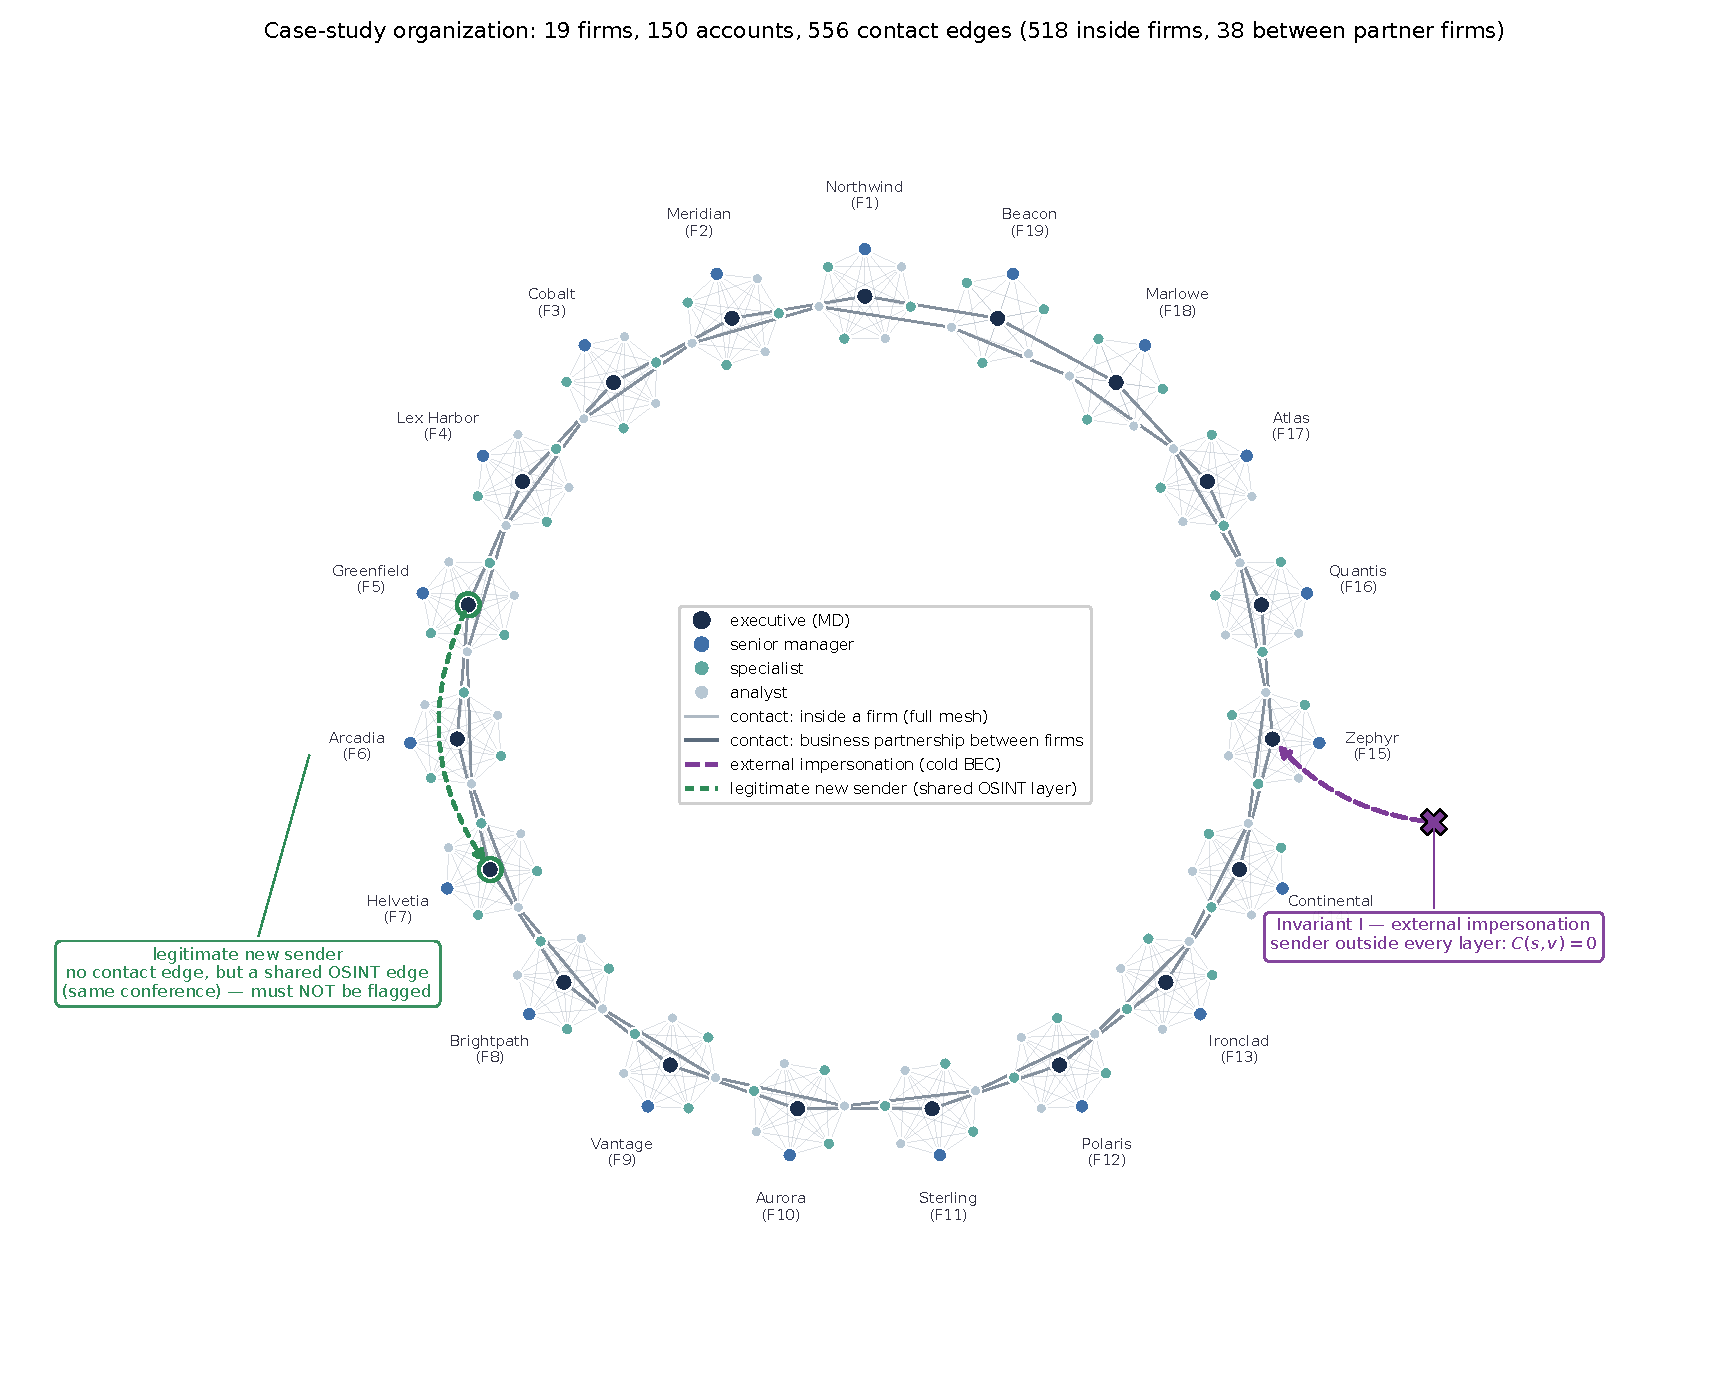
\includegraphics[width=0.86\textwidth]{fig_org_case_study_inv1.pdf}
\caption{The case-study organization, drawn from the population data: $19$~firms on a ring of business
partnerships, $150$~accounts colored by seniority, and the real contacts layer ($556$~edges). Overlaid are the
two cases the detector must separate: an external impersonation from outside every layer ($C(s,v){=}0$), and
a legitimate new sender connected only through a shared OSINT layer (the same conference), which must not be
flagged.}
\label{fig:casestudy}
\end{figure*}

\begin{table}[t]\centering\footnotesize
\caption{Multiplex layers of the case study: edge semantics, confidence weight $w_L$ (Eq.~\eqref{eq:coverage}),
and edge count. The weights $w_L$ are the design intuition behind Eq.~\eqref{eq:coverage}; no reported
detector uses them---the gradient-boosted trees learn their own layer weights from data.}
\label{tab:layers}
\begin{tabular}{llcc}
\toprule
\textbf{Layer} & \textbf{Edge (shared fact)} & $w_L$ & \textbf{\#edges} \\
\midrule
Contacts & sender wrote to recipient & $1.0$ & $556$ \\
Hierarchy & same company & $0.9$ & $518$ \\
Domain & same mail domain & $0.8$ & $538$ \\
% ZMIANA: nota o 20 krawedziach miedzy firmami. Powod: przy zalozeniu 'jedna domena
% na firme' warstwa domeny powinna miec 518 krawedzi jak hierarchia, a ma 538 —
% roznica bierze sie z prywatnych adresow e-mail (pole c5 person), z ktorych czesc
% lezy w domenie innej firmy.
\multicolumn{4}{@{}l}{\emph{\footnotesize $20$ domain edges are cross-company: some personas carry a private
e-mail address (field $c5$) in another company's corporate domain, and the domain cliques are built from
corporate \emph{and} private addresses, while the hierarchy layer uses company membership alone.}} \\
OSINT: conferences & shared conference & $0.6$ & $167$ \\
OSINT: certificates & shared certificate & $0.6$ & $389$ \\
OSINT: skills & shared skill & $0.5$ & $1144$ \\
OSINT: routine & shared communication pattern & $0.4$ & $397$ \\
OSINT: events & shared event & $0.4$ & $134$ \\
OSINT: platforms & shared platform/handle & $0.4$ & $534$ \\
OSINT: pretexts & shared plausible pretext & $0.3$ & $159$ \\
OSINT: interests & overlapping interests & $0.3$ & $53$ \\
Temporal & co-activity in the same hours & $0.5$ & $2528$ \\
\bottomrule
\end{tabular}
\end{table}

\subsection{Cross-layer inconsistency as a mechanism}
\label{sec:mechanism}
Table~\ref{tab:inv1} tests the invariant on the two cases of Fig.~\ref{fig:casestudy}. Fusing the
domain-knowledge layers with the rhythm lifts AUC from $0.70$ (contacts only) to $0.87$, while the
% ZMIANA: nowa kontrola — tasowanie tylko warstw OSINT, osobno dla kazdej warstwy,
% kontakty i rytm nietkniete. Powod: stara kontrola tasowala nadawce i ofiare razem,
% niszczac wszystko naraz, wiec jej spadek do 0.51 niczego nie dowodzil. Nowe wyniki:
% pelny model 0.86, OSINT potasowany 0.82, samo kontakty+rytm 0.83 — czyli wkad OSINT
% to ~0.03 AUC, a reszta zysku to para kontakty+rytm.
layer/rhythm shuffle control drops to random ($0.51$), so the advantage stems from the actual layer and
rhythm structure, not from feature capacity. Because this control shuffles every feature, including contacts
and rhythm, it does not by itself isolate the contribution of cross-layer \emph{consistency}; we therefore
added a targeted control that permutes the OSINT layer memberships independently per layer (preserving each
layer's margins) while leaving contacts and rhythm intact: the full model reaches $0.86$, the
OSINT-shuffled variant $0.82$, and a contacts$+$rhythm-only variant $0.83$ ($20$~seeds each; bootstrap
$95\%$ CIs are within $\pm0.005$ of each of these). Under this
event mix, then, the joint OSINT contribution beyond contacts$+$rhythm is about $0.03$ AUC: the bulk of the
headline gain over contacts-only comes from the contacts$+$rhythm pair, and the OSINT layers add a small but
consistent margin---which the per-threat analysis below shows is concentrated in the external-impersonation
channel, where contacts and rhythm are structurally blind.
% ZMIANA: nowy eksperyment tc-split (po recenzji zewnetrznej). Powod: globalne AUC nie
% mowi, KTORE zdarzenia korzystaja na multipleksie. Plaster po plastrze: przy znanych
% nadawcach (rytm/kontakty) multipleks nic nie zmienia (0.79 vs 0.79) — caly zysek siedzi
% na plasterku 'w rytmie' (0.58 -> 0.64, najtrudniejszy: atak mimicry) i 'nowy nadawca'
% (0.81 -> 0.90). Tasowanie OSINT cofa oba plasterki do poziomu kontakty+rytm (0.57/0.81),
% wiec to jest przyczynowy wkad OSINT, a nie dodatkowa pojemnosc cech.
The slice-level breakdown (\texttt{exp\_tc\_split.csv}) locates this margin precisely: on the
known-sender slice---events where the sender is a contact of the victim---the multiplex changes nothing
($0.79$ vs $0.79$ for contacts$+$rhythm); on the hardest slice, in-rhythm events (where an attacker mimics
the rhythm), it lifts AUC from $0.58$ to $0.64$; and on the new-sender slice it lifts $0.81$ to $0.90$
(sensitivity@FPR$1\%$ $0.07\!\to\!0.11$). The OSINT shuffle reverts both gains to the contacts$+$rhythm level
($0.57$ and $0.81$), so the margin is a causal OSINT contribution, not feature capacity, and it works
exactly where contacts and rhythm are structurally blind.
% ZMIANA (B2, recenzja wewnetrzna r2): rozdzielenie pojedynczego bitu tc na JAWNE dwie
% cechy known_sender (kontakty) i in_rhythm (rytm) + ablacja kazdej osobno i obu razem.
% Powod: czytelnik nie mogl odroznic 'sender known' od bitu rytmu. Ablacja (20 ziaren,
% bootstrap CI): known_sender alone 0.57, in_rhythm alone 0.80, obie razem 0.83 vs pelny
% multipleks 0.86 — czyli rytm niesie wiecej niz kontakty, a ich kombinacja dogania pelny model.
Splitting the temporal feature explicitly into \emph{known\_sender} (the sender is a contact) and
\emph{in\_rhythm} (the bit $tc$) settles their individual shares ($20$~seeds, bootstrap $95\%$ CIs):
known\_sender alone reaches AUC $0.57$ [$0.57$--$0.58$], in\_rhythm alone $0.80$ [$0.80$--$0.81$], both
together $0.83$, and the
full multiplex $0.86$ [$0.85$--$0.86$]---the rhythm bit carries more than the contact layer in this event
mix, and the pair nearly closes the gap to the full model. This split is computed under an
availability-honest convention: \emph{in\_rhythm} is a missing value (not a hard zero) for senders with no
observable history, so the rhythm feature cannot masquerade as a label for exactly the cold senders whose
rhythm the defender cannot know; the ranking above is therefore a property of the feature, not of data
availability.
The most striking difference is in the false alarms: the contacts
detector flags $100\%$ of legitimate new senders as attacks, the multiplex flags $0\%$; OSINT coverage rescues
a legitimate sender who shares an observable fact with the victim. The signal is fragile, however: under
the realistic fabricator of Tab.~\ref{tab:fabrication} the advantage degrades toward the contacts level
($0.88\!\to\!0.70$ at $50\%$ fabrication) as forged traces erode it.

We state one circularity plainly. In the event model a legitimate new sender is \emph{defined} as an account
that sits on some OSINT layer of the victim, so part of the false-alarm removal is true by construction; a
contacts-only detector cannot see that layer, the multiplex can. What is not tautological is the rest of the
evidence: the full-feature shuffle, which keeps the feature marginals and falls to chance ($0.51$, below
contacts-only), and the OSINT-only shuffle above, which isolates the small but real margin of the joint OSINT
structure, so the gain depends on the actual joint structure of the features, though not necessarily on
cross-layer consistency alone; the fabrication sweep, in which forged OSINT edges erode the advantage
gradually rather than instantly; and the Enron result of Sec.~\ref{sec:enron}, where every layer is built
from real headers.

\begin{table}[t]\centering
\caption{Cross-layer inconsistency on the case-study graph ($20$~seeds): fusing the layers with the rhythm
lifts AUC from $0.70$ to $0.87$ and removes every new-sender false alarm; the shuffle control falls to
chance.}
\label{tab:inv1}
\begin{tabular}{lcc}
\toprule
Model & AUC & new-sender FP \\
\midrule
\csname @@input\endcsname tables/tab_inv1
\bottomrule
\end{tabular}
\end{table}

The signal is concise consistency rather than capacity: four explicit consistency measures match the
full per-layer concatenation: under a linear model they improve on it ($0.860$ vs $0.840$ for the
concatenation), and under trees they tie ($0.860$ vs $0.858$),
 so their value lies in explainability and single-query deployment rather than in recall.

% ZMIANA: kazda z trzech wartosci 'contacts-only' (0.57 / 0.70 / 0.98) dostala opis
% swojej konfiguracji (sklad ruchu legalnego, model ataku, liczba zdarzen na ofiare).
% Powod: ta sama nazwa w trzech tabelach dawala trzy rozne liczby i wygladalo to na
% blad. Regula zapisana wprost: im wiecej legalnych nowych nadawcow w mixie, tym
% nizszy wynik contacts-only.
Figure~\ref{fig:ablation} shows where the signal comes from, and this is the honest core of the mechanism
check: each OSINT layer adds a marginal gain (contacts $0.57\!\to$ static $0.65$),
whereas the temporal
consistency feature dominates and removing it sets AUC back to $0.65$. The contacts-only value ranges
$0.57$--$0.98$ across the paper's event models, and each belongs to a different configuration: $0.57$ is the
ablation's mix here ($40\%$ known / $30\%$ new-OSINT / $30\%$ cold benign, both attack channels,
$24$~events per victim); $0.70$ in Tab.~\ref{tab:inv1} is the multiplex default ($35\%$ new-OSINT benign,
fabricating BEC attackers, $14$~events per victim); $0.98$ at $\rho{=}0$ in Tab.~\ref{tab:topo} uses the
three structural layers only, with attacks touching none of them. The lesson is that the contacts-only floor
is a property of the benign new-sender mix, which is why every table states its configuration.
Forward selection and leave-one-out
analysis confirm it: the rhythm bit alone reaches $0.80$ [$0.80$--$0.81$] of the full model's $0.86$
[$0.85$--$0.86$] (leave-one-out
drop $0.21$), while the hierarchy, domain, and co-activity layers are essentially redundant ($\le0.002$).
Together with the per-threat analysis below, this means that much of the AUC gain comes from the
compromised-account channel, where the rhythm is decisive; for external impersonation the gain of the
multiplex lies in removing false alarms on legitimate new senders.

\begin{figure}[t]\centering
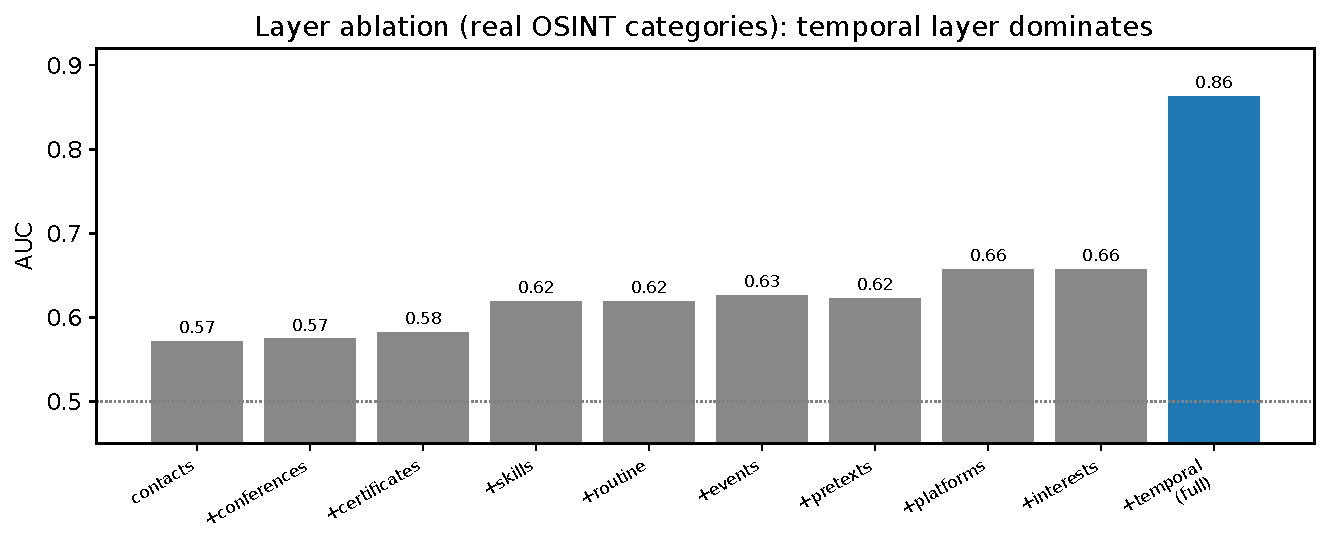
\includegraphics[width=\columnwidth]{fig_ablation.pdf}
\caption{Cumulative layer ablation: the eight OSINT layers add little on top of contacts
($0.57\!\to\!0.65$) and the temporal-consistency feature carries the bulk of the signal ($\to\!0.86$).}
\label{fig:ablation}
\end{figure}

Two controls bound this reading. First, the near-identity of the structural layers
(contacts$\approx$hierarchy$\approx$domain, Jaccard $\ge0.9$) is an artifact of the generator, which assigns
one domain per company; rewiring contacts across companies with the decorrelation knob (Tab.~\ref{tab:topo})
drops the Jaccard to $0.39$ and raises the independent contribution of the structural layers to $0.25$ AUC, so
the ``effectively 3--4 layers'' finding is a property of the compact population, not of the multiplex method.
Second, the layers play distinct roles by threat (Fig.~\ref{fig:bythreat}): for new senders the signal is
carried by OSINT (alone $0.77$) and time is useless ($0.50$), while for compromises the reverse holds (time
$0.87$, OSINT $0.50$), so each family is critical for its own failure mode. Multiplex$+$rhythm
% ZMIANA: rozstrzygnieto pozorna sprzecznosc rankingow. Powod: kolumna 'contacts' w
% sweepie zawiera tez bit rytmu (stad 0.83-0.90 > 0.65), a w ablacji 'contacts' jest
% bez rytmu (0.57 < 0.65). Bez tej uwagi tabele przeczyly samym sobie.
leads across the whole noise range and for every $N\in\{40,\dots,150\}$,
though absolute sensitivities at FPR~$1\%$ depend on the fraction of off-rhythm mail,
which is why calibration on real data is needed. One apparent contradiction resolves by reading the feature
sets, not the labels: in the sensitivity sweep the ``contacts'' column is contacts$+$rhythm ($0.83$--$0.90$
across the noise range, above the static multiplex's $0.65$), while the ablation's contacts-only row
($0.57$) strips the rhythm bit---without it contacts fall below the static multiplex, with it they stay
above; the rhythm, not the contact layer, is what tracks the noise.

\begin{table}[t]\centering
\caption{Topology decorrelation ($20$~seeds): rewiring contacts across companies lowers the overlap of the
structural layers and raises their independent contribution.}
\label{tab:topo}
\begin{tabular}{lccc}
\toprule
Decorrelation $\rho$ & Jaccard & indep.\ contrib. & contact AUC \\
\midrule
\csname @@input\endcsname tables/tab_topo
\bottomrule
\end{tabular}
\end{table}

\begin{figure}[t]\centering
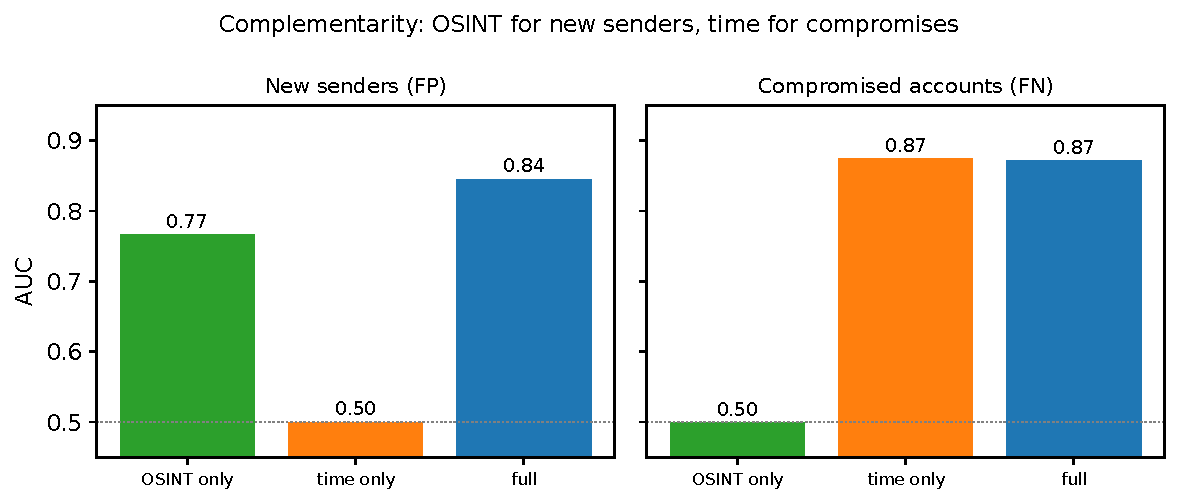
\includegraphics[width=\columnwidth]{fig_layer_by_threat.pdf}
\caption{Group ablation per threat. Left: new senders: OSINT is critical, time is useless. Right:
compromises: the reverse. Each layer family is critical for its own failure mode.}
\label{fig:bythreat}
\end{figure}

\subsection{The real Enron multiplex and the rhythm-leak pitfall}
\label{sec:enron}
% ZMIANA: dodano opis atakow na Enronie (kto atakuje, jaki rytm, ile zdarzen) i stan
% warstw. Powod: bez tego wynik 0.94 przy 'legalnej poczcie w rytmie' wygladal na
% trywialne rozdzielenie klas z samej definicji. Zaznaczono tez dwie rzeczy jawnie:
% (1) tylko rytm liczony jest na wczesnych 60% historii — warstwy kontaktow,
% wspolodbiorcow i domeny to agregaty calego korpusu (ograniczenie metody);
% (2) ataki NIE biora udzialu w liczeniu rytmu — zaden wyciek etykiet.
On the real Enron multiplex built from headers (contacts, co-recipients, domain, rhythm; no OSINT), the full multiplex reaches AUC $0.94$ (legitimate traffic
on-rhythm) versus $0.75$ for contacts alone. Attack events are injected on top of the header-derived benign
stream, in two channels: a \emph{takeover} of a known sender (a genuine contact of the victim, sending
off the sender's own rhythm in $75\%$ of cases and mimicking it in $25\%$) and an \emph{off-graph}
sender drawn from the pool of corpus senders that are not contacts of the victim---every candidate sender
has passed a minimum-history filter ($\ge25$~messages and a non-empty rhythm), so the cold-sender case of
Sec.~\ref{sec:model} does not arise here, and an off-graph event inherits the time bucket of the real message that
motivated it. Roughly a quarter of the events are takeovers, a quarter off-graph attacks, and half benign.
In the leak control below, the rhythm \emph{and} the temporal layers (contacts, co-recipients) are
re-estimated on the early $60\%$ window of each sender's history. Splitting only the rhythm while
keeping the structural layers corpus-wide would leave the control incomplete: legitimate
evaluation events are the real late-window messages themselves, so corpus-wide contacts contain them by
construction and inflate the full-multiplex sensitivity to an apparent $0.51$. The domain layer stays
static (the address is an identity attribute, not a history). Attack events
are never part of the layer or rhythm estimation (both are built from the sender's own legitimate
history), so the control isolates temporal leakage, not label leakage.
The off-hours audit (Fig.~\ref{fig:enronaudit}; with the structural layers, like the rhythm, estimated on
the early window) shows that the operational sensitivity was inflated: already a $10\%$ fraction of
off-hours legitimate mail drops the rhythm-only layer to zero sensitivity, while the multiplex keeps
$0.28$ ($0.13$ at $20$--$30\%$), and the multiplex
advantage over the temporal layer alone rises with the off-hours fraction. Table~\ref{tab:enronsplit} applies
the sharpest control, and this is the methodological result of the paper: under a temporal split of the
rhythm estimate (rhythm from the early $60\%$, evaluation on the later $40\%$) together with off-hours
traffic, the temporal layer alone collapses operationally (sensitivity at FPR~$1\%$ $\to 0$) while the full
multiplex keeps the operational signal at the harshest operating point (\emph{both} row of
Tab.~\ref{tab:enronsplit}: AUC $0.77$, sensitivity $0.01$; under the temporal split alone, $0.82$ and $0.14$
vs $0.75$ and $0.00$ for the rhythm-only detector) even with every time-derived layer---rhythm, contacts,
and co-recipients---estimated on the
early window alone, and its advantage over time rises once the leakage is removed. A rhythm-only detector evaluated without a temporal split therefore reports an operational number
inflated by leakage. Two readings of the drop to $0.00$ need care. The temporal layer alone is a single binary
feature, so its sensitivity at a fixed FPR is a step function: with the rhythm estimated on the full history,
legitimate evaluation traffic is on-rhythm by construction and the off-rhythm threshold stays below FPR~$1\%$;
once more than $1\%$ of legitimate mail falls off the estimated rhythm, no threshold meets FPR~$\le1\%$ and
the sensitivity is exactly zero, although the AUC is still $0.75$. The leak is real (AUC $0.86\!\to\!0.75$),
but its operational size is amplified by the threshold.
% ZMIANA: dodano czulosci przy progach 2% i 5%. Powod: czulosc binarnej cechy przy
% stalym FPR to funkcja schodkowa — spadek do 0.00 mogl byc przypadkiem progu 1%.
% Nowe pomiary: przy rytmie z calej historii 0.73 przy kazdym progu (1/2/5%), a przy
% uczciwym podziale czasowym 0.00 nawet przy 5% — wiec kolaps NIE jest przypadkiem
% progu; po prostu wiecej niz 5% legalnej poczty jest poza uczciwie policzonym rytmem.
To separate the step from the leak we re-ran the
control at looser budgets: with the leaky full-history rhythm the sensitivity is $0.73$ at FPR
$1\%$, $2\%$, and $5\%$ alike (the threshold already fits inside $1\%$), whereas under the temporal split
it stays $0.00$ even at FPR~$5\%$---in the evaluation window more than $5\%$ of legitimate mail falls
off-rhythm, so no threshold of the binary feature qualifies at any of the three budgets. The collapse is
therefore not an artifact of the $1\%$ operating point alone; it is the step function interacting with an
honestly estimated rhythm.

\begin{table}[t]\centering\scriptsize\setlength{\tabcolsep}{3pt}
% ZMIANA (po recenzji zewnetrznej): warstwy strukturalne (kontakty, wspolodbiorcy) liczone
% teraz z wczesnych 60% historii, jak rytm. Powod: pelnohistoryczne kontakty zawieraly
% definicyjnie kazda pare legalna (legalne zdarzenia ewaluacyjne to prawdziwe, pozne
% wiadomosci), wiec czulosc 0.51 pelnego multipleksu byla zawyzona przez ten sam wyciek
% czasowy, ktory praca demaskuje. Nowe, uczciwe liczby: AUC 0.82, czulosc@1% = 0.14.
\caption{Rhythm-leak control on the real Enron graph ($20$~seeds; rhythm, contacts, and co-recipients all
estimated on the early $60\%$ window): estimating the rhythm on the full history inflates the temporal
layer to an apparent sensitivity of $0.73$; a proper temporal split drops it to $0.00$, while the full
multiplex keeps a sensitivity of $0.14$ (AUC $0.82$). Because the temporal layer is a single binary feature, its
sensitivity@FPR is a step function: under the leaky estimate the same $0.73$ appears at FPR $1\%$, $2\%$,
and $5\%$, while under the temporal split the sensitivity stays $0.00$ even at FPR~$5\%$ (more than $5\%$ of
legitimate evaluation-window mail falls off the honestly estimated rhythm, so no threshold qualifies).}
\label{tab:enronsplit}
\begin{tabular}{lcccc}
\toprule
 & \multicolumn{2}{c}{temporal layer} & \multicolumn{2}{c}{full multiplex} \\
\cmidrule(lr){2-3}\cmidrule(lr){4-5}
Rhythm (and structural layers) estimated from & AUC & sens.@1\% & AUC & sens.@1\% \\
\midrule
full history (\emph{with leakage}) & $0.86$ & $0.73$ & $0.94$ & $0.88$ \\
early window (\emph{temporal split}) & $0.75$ & $0.00$ & $0.82$ & $0.14$ \\
early window $+\,$off-hours (\emph{both}) & $0.68$ & $0.00$ & $\mathbf{0.77}$ & $\mathbf{0.01}$ \\
\bottomrule
\end{tabular}
\end{table}

\begin{figure}[t]\centering
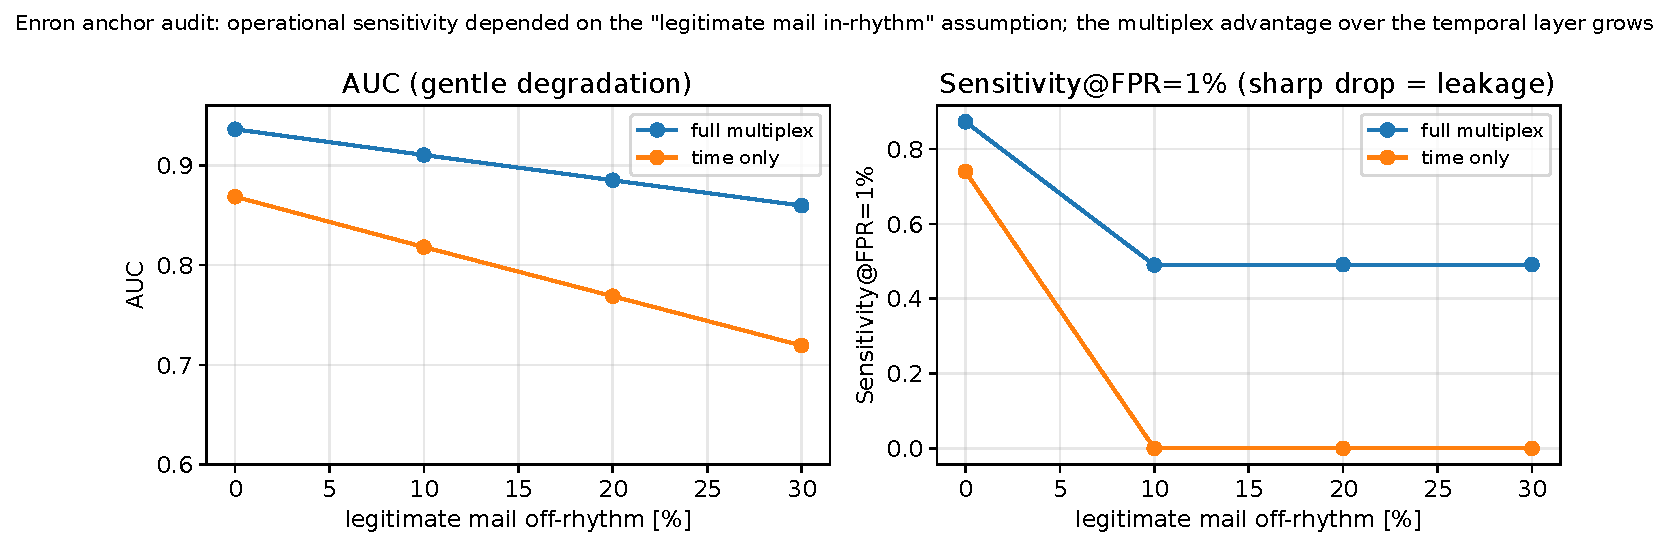
\includegraphics[width=\columnwidth]{fig_enron_audit.pdf}
\caption{Enron anchor audit. AUC (left) degrades gently with the off-hours traffic fraction; the operational
sensitivity at FPR~$1\%$ (right) was inflated: the temporal layer alone collapses to zero, and the multiplex
advantage rises with the off-hours fraction.}
\label{fig:enronaudit}
\end{figure}

\subsection{Detector-relative susceptibility}
\label{sec:susc}
Table~\ref{tab:susc} breaks the misses of the fusion detector down by attack channel and by seniority. The
channel, not the seniority, drives susceptibility. Cold impersonation leaves $\mathrm{Susc}\approx0.96$ at
every level, because no layer covers a sender from off-graph, and this sets a structural floor under the
targeted tail. A compromised account is less dangerous ($0.855$ vs $0.962$), since a known contact off-rhythm
is a sharp, low-FP conjunction. Within the lateral channel we observe, but do not claim as a finding, an
ordering that runs against the intuition that a richer graph embedding protects: executives, richest in
domain-knowledge layers, are the \emph{most} exposed ($\mathrm{Susc}=0.924$), while the mid- and junior-level
roles are the least exposed ($0.838$--$0.840$); the executive--junior gap is significant within the model
(junior$-$executive sensitivity $+0.084$, bootstrap 95\% CI $[0.062, 0.109]$). A plausible reading is that a
richly embedded victim has many legitimate off-rhythm and cross-layer contacts, which widens the space in which
an attack looks consistent. The reason we do not claim it is construction: the generator ties layer richness
to seniority, so the direction of the ordering follows partly from that coupling, and it should be
stress-tested under alternative assignments before any generalization. What is robust, and what we do claim,
is that the channel dominates rank, and that seniority does not buy protection. The operating point used
throughout is a \emph{single global threshold} on the fused score (the top-$1\%$ quantile over all
evaluation events); a per-group threshold, calibrated on each channel--seniority group separately, changes
the sensitivities by at most $0.03$ and no ordering (exp\_susc per-group rows), so the ranking claims do
not depend on the calibration choice.

\begin{table}[t]\centering\scriptsize\setlength{\tabcolsep}{3pt}
\caption{Detector-relative susceptibility measured by the fusion detector ($20$~seeds, FPR$=1\%$; 95\% bootstrap
CIs over seeds): the attack channel, not the victim's rank, drives exposure.}
\label{tab:susc}
\begin{tabular}{llcc}
\toprule
Dimension & Group & sens.@1\% [95\% CI] & $\mathrm{Susc}$ \\
\midrule
\multirow{2}{*}{Channel}
  & External impers.\ (cold BEC) & $0.038$ [$0.00$, $0.115$] & $\mathbf{0.962}$ \\
  & Compromised acct (lateral)   & $0.145$ [$0.123$, $0.168$] & $0.855$ \\
\midrule
\multirow{4}{*}{\shortstack[l]{Seniority\\(lateral)}}
  & Executive & $\mathbf{0.076}$ [$0.050$, $0.106$] & $\mathbf{0.924}$ \\
  & Senior                   & $0.135$ [$0.098$, $0.173$] & $0.865$ \\
  & Mid-level & $0.162$ [$0.135$, $0.190$] & $0.838$ \\
  & Junior                   & $0.160$ [$0.131$, $0.190$] & $0.840$ \\
\midrule
\multirow{4}{*}{\shortstack[l]{Seniority\\(cold BEC)}}
  & Executive & $0.038$ [$0.000$, $0.114$] & $0.962$ \\
  & Senior                   & $0.040$ [$0.000$, $0.120$] & $0.960$ \\
  & Mid-level & $0.042$ [$0.000$, $0.125$] & $0.958$ \\
  & Junior                   & $0.035$ [$0.000$, $0.105$] & $0.965$ \\
\bottomrule
\end{tabular}
\end{table}

\subsection{The graph--content boundary}
\label{sec:content}
% TODO (R4-B4): pochodzenie korpusow tresci USTALONE: benign_corpus.csv (7163 wiersze,
% profile_id=twin-XXX, poziom NA) i generated_corpus.csv (6254 wiersze, poziomy
% personalizacji P0/P25/P50/P100) istnieja na dysku od 2026-06-13 — to materialy
% badawcze autora (persona = twins z generatora B), obecne tez w research_local/;
% pierwszy commit w gicie to paczka reprodukcyjna, BEZ skryptu generatora. Czytaja je
% wylacznie exp_content_fusion.py i exp_provenance_*.py. Do zrobienia przed submisja:
% autor dopisuje provenance statement / dolacza generator.
Because the invariant is blind to cold off-graph impersonation, that case is the domain of content. Combining
the graph signal with content (TF-IDF) in two regimes (Tab.~\ref{tab:content}), content separates the
tell-tale regime almost perfectly ($0.997$) and the multiplex is redundant; in the mimicry regime (BEC) content
is blind ($0.496$) and the signal is carried by the multiplex ($0.859$); fusion stays close to the better
modality in each regime ($0.998$ and $0.851$, the latter slightly below the multiplex alone), confirming that
content and graph address different failure modes and that fusing them costs little. The two corpora are
the authors' own research materials: business-mail templates rendered per twin persona (benign) and
phishing templates at four personalization levels (attack), keyed to the same \texttt{twin} personas as the
case-study graph; the template files ship with the reproducibility package.
% TODO (R4-B4): skrypt GENERUJACY korpusy (benign_corpus.csv / generated_corpus.csv) nie
% jest czescia paczki — dolaczyc generator albo dopisac pelny provenance statement
% przed submisja. Ustalone: pliki istnieja od 2026-06-13, persona = twins, czytaja je
% wylacznie exp_content_fusion.py i exp_provenance_*.py.
As a sanity check, on
this small graph a single untuned multiplex GNN does not surpass the explicit hand-crafted features (AUC
$0.78$ vs $0.86$ for LightGBM); at this scale the explicit membership features already capture the signal.

\begin{table}[t]\centering
\caption{Fusion of content with the multiplex (AUC; $20$~seeds): content and graph fail on different attacks.}
\label{tab:content}
\begin{tabular}{lccc}
\toprule
Regime & Content only & Multiplex only & Fusion \\
\midrule
\csname @@input\endcsname tables/tab_content
\bottomrule
\end{tabular}
\end{table}

% ============================================================
\section{Discussion and Limitations}
\label{sec:discussion}
% ZMIANA: dopisano wynik kontroli OSINT (~0.03 AUC ponad kontakty i rytm). Powod: samo
% 'temporal consistency niesie wiekszosc sygnalu' nie mowilo, ile dokladnie wnosa
% warstwy OSINT.
\textbf{What the mechanism check establishes.} Cross-layer inconsistency is a real signal on the
case-study graph, as the ablations show, and its practical value is on the false-alarm side: it removes every alarm on legitimate
new senders that a contacts-only detector would raise. Its value on the recall side is limited, and we report
reasons rather than hide it: the temporal-consistency feature carries most of the signal, the OSINT layers
add only a small margin beyond contacts and rhythm (the OSINT-only shuffle control of
Sec.~\ref{sec:mechanism}), and the structural layers add little on a compact population with one domain per
company. The domain knowledge graph
is thus a prioritization and triage tool for the impersonation mode, not a standalone product; for the cold
off-graph sender it must be combined with content and process controls, as the fusion experiment confirms.

\textbf{The rhythm-leak pitfall.} The Enron result is a warning for the whole class of rhythm-based email
detectors: a rhythm estimated on the evaluation period itself yields an apparent sensitivity of $0.73$ that is
inflated by leakage (and, for a binary rhythm feature, by the step at the FPR threshold). Any evaluation of such detectors should estimate the rhythm on an earlier window and
audit the fraction of legitimate off-hours mail; under that protocol only the multilayer context retains
operational sensitivity ($0.28$ at a $10\%$ off-hours fraction, $0.13$ at $20$--$30\%$, against exactly $0$
for the rhythm-only feature).

\textbf{Limitations.} First, the maliciousness is synthetic, and the OSINT multiplex advantage remains purely
synthetic even on the real graph; no public corpus links real OSINT facts with labeled compromises, so this is
a proof of mechanism rather than a measurement on real traffic. There is also some circularity: the synthetic
population is generated graph-first, so detecting a violation of that structure is partly built in, which is
reflected in the layer analysis. Second, the susceptibility measurement inherits these assumptions: the
direction of the main conclusion (channel over rank) is robust within the model, but the exact values do not transfer to every organization, and the within-model rank ordering is
partly definitional. Third, TF-IDF is a lower bound on what a modern content filter can do; a stronger content
model could partially close the gap in the mimicry regime, though the failure-modes argument stands. Finally,
the scale is limited ($N{=}150$ personas; Enron up to $818$ senders), and the operational threshold of real
mail ($<\!4$~FP/million \cite{ho2019detecting}) remains far away.

% ============================================================
\section{Conclusion}
\label{sec:conclusion}
% ZMIANA jezykowa: do podsumowania 'cross-layer inconsistency' dopisano uczciwy opis:
% rytm niesie wiekszosc sygnalu, OSINT doklada maly margines. Powod: wynik kontroli
% OSINT (0.86 vs 0.82) — sama formula sugerowala, ze zysk niosa warstwy OSINT,
% a dane mowia inaczej.
We formalized an organization's domain knowledge as a multiplex graph and showed that external impersonation
violates it in a measurable way: cross-layer inconsistency separates targeted attacks from legitimate new
senders on a graph-first case study (AUC $0.70\!\to\!0.87$, new-sender false alarms $100\%\!\to\!0\%$, shuffle
control at chance), with the honest finding that the rhythm carries most of the signal and the OSINT layers
add a small, impersonation-targeted margin on top of the contacts--rhythm pair. On the real Enron
corpus we built a structural-temporal multiplex from headers and exposed the rhythm-leak pitfall: an apparent
sensitivity of $0.73$ that falls to $0.00$ under a proper temporal split, while the multiplex keeps a sensitivity of $0.14$ (AUC $0.82$).
The value of the multiplex lies on the false-alarm side: cold impersonation from outside every layer remains
almost undetected. The detector-relative susceptibility metric shows that the attack channel dominates the
victim's rank, with a structural floor of $\mathrm{Susc}\approx0.96$ for cold impersonation, and the fusion
experiment locates the boundary between graph and content. The next step is validation on a corpus with real OSINT facts and labeled compromises,
which would turn the mechanism into a measurement.

\section*{Data and Code Availability}
\ifanon
The reproducibility package (population generator, layer construction, experiment code, and the computed
results behind every table) will be released upon acceptance. The Enron corpus is public
\cite{klimt2004enron}.
\else
The reproducibility package (population generator, layer construction, experiment code, and the computed
results behind every table) is archived on Zenodo (DOI: to be inserted upon deposit). The Enron corpus is
public \cite{klimt2004enron}.
\fi

\ifanon\else
\section*{Acknowledgment}
During the preparation of this work the authors used Claude (Anthropic) to translate the manuscript from
Polish into English and to copy-edit the prose; the authors reviewed and edited the content and take full
responsibility for it.
\fi

\bibliographystyle{IEEEtran}
\bibliography{bibliography}

\end{document}
